\documentclass[11pt]{amsart}
\textwidth 6.3in

\evensidemargin=-0.1cm \oddsidemargin=-0.1cm

\textheight 8.1in

\usepackage{tikz-cd}

\begin{document}


\begin{center}
\huge HW 1 \\
50 points \\

\Large Posted Tuesday, September 2

\Large Due Thursday, September 18 at midnight

\normalsize
\end{center}


Note: Lecture 2 covers material for 1-4 (except for 3(e)). Lectures 3 and 4 cover 5 and 6. Submit solutions in file \texttt{HW1Solutions.pdf}. Submission size limit in Submitty is set to 2.5MB.

\vspace{0.15in}

\noindent{\bf Problem 1.} Describe the languages denoted by the following regular expressions using the highest level characterization possible.


\begin{enumerate}

\item[(a)] (0.5pts) $\texttt{a(a|b)}^*\texttt{a}$

\item[(b)] (0.5pts) $\texttt{((}\epsilon \texttt{|a)b}^\texttt{*}\texttt{)}^\texttt{*}$

\item[(c)] (0.5pts) $\texttt{(a|b)}^*\texttt{a(a|b)(a|b)}$

\item[(d)] (0.5pts) $\texttt{a}^\texttt{*}\texttt{ba}^\texttt{*}\texttt{ba}^\texttt{*}$

\item[(e)] (3pts) $\texttt{(aa|bb)}^\texttt{*}\texttt{((ab|ba)(aa|bb)}^\texttt{*}\texttt{(ab|ba)(aa|bb)}^\texttt{*}\texttt{)}^\texttt{*}  \texttt{((ab|ba)(aa|bb)}^\texttt{*}\texttt{a|b)} $

\end{enumerate}

\vspace{0.5cm}

\begin{enumerate}

\item[(a)] All strings of a's and b's that start and end with an a. Ex: $\{aa, aba, aaaa, abba,...\}$

\item[(b)] All possible strings of a's and b's including the empty string. Ex: 

$\{\epsilon, a, b, ab, ba, aa, bb, aaa,...\}$

\item[(c)] All strings of a's and b's whose third to last character is a 'a'. Ex: 
\item[] 
$\{aaaa, aaab, aaba, aabb, baaa, baab...\}$

\item[(d)] All strings of a's and b's that contain exactly two b's. The two b's can be right next to each other or separated by any number of a's. Ex:

$\{bb, abb, bab, bba, abab, ababa, ...\}$

\item[(e)] All strings of a's and b's that contains an even number of a's and an odd number of b's. 
\item[] 
Ex: $\{b, aab, abb, aba, aaabb, ababb,...\}$

\end{enumerate}

\newpage

\vspace{0.5cm}

\noindent{\bf Problem 2}. The following grammar generates binary strings that have \emph{even} values. $S$ is the start symbol. 
 
\begin{enumerate}

\item[] $S\rightarrow A$ 

\item[] $A\rightarrow B\ \texttt{0} \mid A\ \texttt{0} \mid \texttt{0}$

\item[] $B\rightarrow A\ \texttt{1} \mid B\ \texttt{1} \mid \texttt{1}$

\end{enumerate}

\vspace{.05in}

Your task is to construct a similar grammar that generates strings with values divisible by 3. 

\vspace{.05in}

\begin{enumerate}

\item [(a)] (3pts) Fill in the blanks to complete the grammar:

\begin{enumerate}

\item[] $S\rightarrow A$

\item[] $A\rightarrow A\ \texttt{0} \mid B\ \texttt{1} \mid \texttt{0}$

\item[] $B\rightarrow C\ \texttt{0} \mid A\ \texttt{1} \mid \texttt{1} $

\item[] $C\rightarrow B\ \texttt{0} \mid C\ \texttt{1} $

\end{enumerate}


\vspace{0.25cm}

\item[(b)] (1pts) Using your grammar, show a derivation that generates 21 in binary notation.

\vspace{0.25cm}

21 in binary is 10101. One possible derivation is:

\vspace{0.25cm}

\begin{enumerate}

\item[] $S\Rightarrow A$

\item[] $\ \ \  \Rightarrow B1$ ($A \rightarrow B1$)

\item[] $\ \ \  \Rightarrow C01$ ($B \rightarrow C0$)

\item[] $\ \ \  \Rightarrow C101$ ($C \rightarrow C1$)
 
\item[] $\ \ \  \Rightarrow B0101$ 

\item[] $\ \ \  \Rightarrow 10101$

\end{enumerate}

\vspace{0.25cm}

\item[(c)] (4pts) Prove that all binary strings generated by your grammar have values divisible by 3. ({\it{Note: Use induction on the number of nodes in the parse tree.}})

\vspace{0.25cm}

\textbf{Induction Hypothesis:} Assume that for any terminal string $w$,

\vspace{0.25cm}

1. If $w$ is derived from A, then val($w$) ($\equiv 0 \mod 3$)

2. If $w$ is derived from B, then val($w$) ($\equiv 1 \mod 3$)

3. If $w$ is derived from C, then val($w$) ($\equiv 2 \mod 3$)

\vspace{0.25cm}

Where val($w$) is the integer value of the binary string $w$.

\vspace{0.25cm}

\textbf{Base Case:} Length of $w$ ($|w|$)= 1. The only derivable strings of length 1 from our grammer is

\vspace{0.25cm}

1. $w$ = 0 from A val($w$) = 0 $\equiv 0 \mod 3$, holds true with our hypothesis.

2. $w$ = 1 from B. val($w$) = 1 $\equiv 1 \mod 3$, holds true with our hypothesis.

3. No string of length 1 can be derived from C. which still holds true with our hypothesis.

\vspace{0.25cm}

\textbf{Inductive Step:} Assumiming that the three statements of our induction hypothesis holds for all terminal strings of length $\le$ k. Let $w$ be the terminal string of length k + 1 derived from A, B or C. We consider each production used to get k + 1 length of $w$ and check if each holds true to the induction hypothesis.

\vspace{0.25cm}

1. For A $ \rightarrow A0$. Suppose A derives string $x$ of length k + 1. Appending $0$ gives string $x0$ whose value is val(x0) = 2*val(x). By our inductive hypothesis, val(x) $\equiv 0$. Therefore, val(x0) $\equiv 2*0 \equiv 0 \mod 3$. Holds true.

2. For A $ \rightarrow B1$. Suppose B derives string $y$ of length k + 1. Appending $1$ gives string $y1$ whose value is val(y1) = 2*val(y) + 1. By our inductive hypothesis, val(y) $\equiv 1$. Therefore, val(y1) $\equiv 2*1 + 1 \equiv 3 \equiv 0 \mod 3$. Holds true.

3. For A $ \rightarrow 0$. This is our base case which we have already shown to hold true.

4. For B $ \rightarrow C0$. Suppose C derives string $z$ of length k + 1. Appending $0$ gives string $z0$ whose value is val(z0) = 2*val(z). By our inductive hypothesis, val(z) $\equiv 2$. Therefore, val(z0) $\equiv 2*2 \equiv 4 \equiv 1 \mod 3$. Holds true.

5. For B $ \rightarrow A1$. Suppose A derives string $x$ of length k + 1. Appending $1$ gives string $x1$ whose value is val(x1) = 2*val(x) + 1. By our inductive hypothesis, val(x) $\equiv 0$. Therefore, val(x1) $\equiv 2*0 + 1 \equiv 1 \mod 3$. Holds true.

6. For B $ \rightarrow 1$. This is our base case which we have already shown to hold true.

7. For C $ \rightarrow B0$. Suppose B derives string $y$ of length k + 1. Appending $0$ gives string $y0$ whose value is val(y0) = 2*val(y). By our inductive hypothesis, val(y) $\equiv 1$. Therefore, val(y0) $\equiv 2*1 \equiv 2 \mod 3$. Holds true.

8. For C $ \rightarrow C1$. Suppose C derives string $z$ of length k + 1. Appending $1$ gives string $z1$ whose value is val(z1) = 2*val(z) + 1. By our inductive hypothesis, val(z) $\equiv 2$. Therefore, val(z1) $\equiv 2*2 + 1 \equiv 5 \equiv 2 \mod 3$. Holds true.

\vspace{0.25cm}

And thus, by induction, we have show that our induction hypothesis holds true for all terminal strings derived from each of our productions from our grammer for lengths k + 1. 

\item[(d)] (4pts) Prove that your grammar generates all binary strings with values divisible by 3. 

\vspace{0.25cm}

Let $w$ be all binary strings with $val(w)$ divisible by 3. If we look at the DFA for remainder mod 3 while reading $w$ from left to right. Each spot over is mirrored by a production in the grammer, giving us a derivation of $w$ from S, our start point. Hence, the grammer generates all binary strings with values divisible by 3.

\vspace{0.25cm}

\begin{center}
	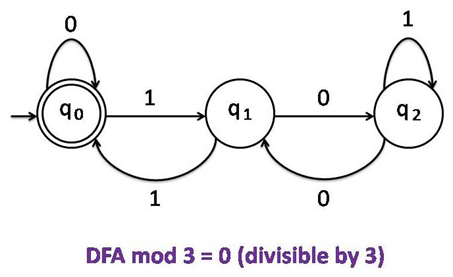
\includegraphics[width=0.6\textwidth]{image(886).png}
\end{center}

\end{enumerate}

\vspace{.15in}

\newpage

\noindent{\bf Problem 3.} Consider the grammar 

\vspace{0.05in}

\begin{enumerate}

\item[(1)] $S\rightarrow \texttt{a}\ S \ \texttt{b}\ S$

\item[(2)] $S\rightarrow \texttt{b}\ S \ \texttt{a}\ S$

\item[(3)] $S\rightarrow \epsilon $

\end{enumerate}

\vspace{0.05in}

\begin{enumerate}

\item[(a)] (1pts) Show that the grammar is ambiguous by constructing two different leftmost derivations for a string. Use the shortest string possible. 

\vspace{0.25cm}

1st Derivation:

\vspace{0.25cm}

\begin{enumerate}
	\item [] $S \Rightarrow aSbS$
	\item [] $\ \ \ \Rightarrow abSaSbS$
	\item [] $\ \ \ \Rightarrow ab\epsilon aSbS$
	\item [] $\ \ \ \Rightarrow abaSbS$
	\item [] $\ \ \ \Rightarrow aba\epsilon bS$
	\item [] $\ \ \ \Rightarrow ababS$
	\item [] $\ \ \ \Rightarrow abab\epsilon$
	\item [] $\ \ \ \Rightarrow abab$
\end{enumerate}

\vspace{0.25cm}

2nd Derivation:

\vspace{0.25cm}

\begin{enumerate}
	\item [] $S \Rightarrow aSbS$
	\item [] $\ \ \ \Rightarrow a\epsilon bS$
	\item [] $\ \ \ \Rightarrow abS$
	\item [] $\ \ \ \Rightarrow abaSbS$
	\item [] $\ \ \ \Rightarrow aba\epsilon bS$
	\item [] $\ \ \ \Rightarrow ababS$
	\item [] $\ \ \ \Rightarrow abab\epsilon$
	\item [] $\ \ \ \Rightarrow abab$
\end{enumerate}

\vspace{0.25cm}

Constructed the string "abab" in in two different leftmost derivations, showing that the grammer is ambiguous.

\vspace{0.25cm}

\item[(b)] (1pts) Construct the corresponding rightmost derivations for the string from (a).

\vspace{0.25cm}

1st Derivation:

\vspace{0.25cm}

\begin{enumerate}
	\item [] $S \Rightarrow aSbS$
	\item [] $\ \ \ \Rightarrow aSb\epsilon$
	\item [] $\ \ \ \Rightarrow aSb$
	\item [] $\ \ \ \Rightarrow abSaSb$
	\item [] $\ \ \ \Rightarrow abSa\epsilon b$
	\item [] $\ \ \ \Rightarrow abSab$
	\item [] $\ \ \ \Rightarrow ab\epsilon ab$
	\item [] $\ \ \ \Rightarrow abab$
\end{enumerate}

\newpage
2nd Derivation:

\vspace{0.25cm}

\begin{enumerate}
	\item [] $S \Rightarrow aSbS$
	\item [] $\ \ \ \Rightarrow aSbaSbS$
	\item [] $\ \ \ \Rightarrow aSbaSb\epsilon $
	\item [] $\ \ \ \Rightarrow aSbaSb$
	\item [] $\ \ \ \Rightarrow aSba\epsilon b$
	\item [] $\ \ \ \Rightarrow aSbab$
	\item [] $\ \ \ \Rightarrow a\epsilon bab$
	\item [] $\ \ \ \Rightarrow abab$
\end{enumerate}

\vspace{0.25cm}

\item[(c)] (2pts) Construct the corresponding parse trees.

\begin{center}
	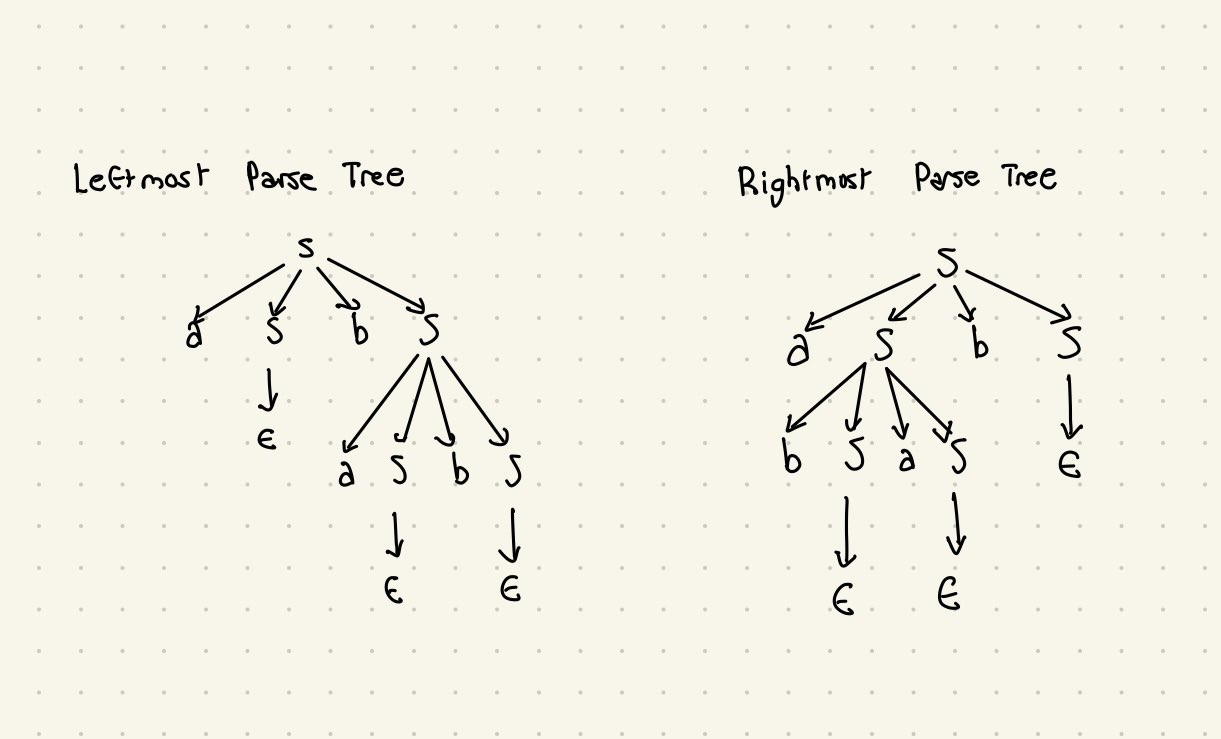
\includegraphics[width=0.6\textwidth]{IMG_0078.jpg}
\end{center}

\item[(d)](3pts) One can see that the grammar generates strings with equal number of \texttt{a}'s and \texttt{b}'s. Does it generate \emph{all} such strings? ({\it{Note: You do not need to write a full formal proof. If you answer YES, outline an inductive argument. If you answer NO, show a string with equal number of \texttt{a}'s and \texttt{b}'s that cannot be generated by the grammar.}})

\vspace{0.25cm}

Yes, the grammar does generate all strings with an equal number of a's and b's.

\vspace{0.25cm}

We can prove this by induction.

\vspace{0.25cm}

It'll look something like this:

\vspace{0.25cm}

\textbf{Induction Hypothesis:} Assume that every string with exactly k a's and k b's for some k $\ge$ 0 can be generated by the grammer.

\textbf{Base Case:} For n = 0, the empty string $\epsilon$ can be generated by rule 3. 0 a's and 0 b's. Holds true to our hypothesis.

\textbf{Inductive Step:} Let $w$ be any nonempty string with n = k + 1 a's and b's, check each production of our grammer to make sure our hypothesis holds true for 2(k + 1) length string generated by our production holds true to our induction hypothesis.

\vspace{0.25cm}

1. For production 1, $S \rightarrow aSbS$. Any string $w$ generated by this production must start with an 'a' and have a corresponding 'b' that matches it. All other productions of S will follow in the same manner, with S only either able to transform into bSaS or $\epsilon$. By our inductive hypothesis, all strings generated by S will have an equal number of a's and b's. Hence, any string $w$ generated by this production will have an equal number of a's and b's.

2. For production 2, $S \rightarrow bSaS$. Any string $w$ generated by this production must start with an 'b' and have a corresponding 'a' that matches it. Same case here.

3. For production 3, $S \rightarrow \epsilon$. This is our base case which we have already shown to hold true.

\item[(e)] (5pts) Finally, write a recursive descent parser with backtracking in Python. Include function \texttt{dfparse(s:str) -> list[int]} that takes a string and returns the list of productions the parser applied (if the parse succeeded). An unusual requirement is that your backtracking parser tries the $S$ productions in reverse order: it first tries (3), then (2), then (1). Include the function in file \texttt{backtrack.py} and turn in Submitty. You may assume that we'll test with string inputs only. A few sample runs are included:

\begin{verbatim}

python3 -i backtrack.py 
>>> dfparse('')
[3] 

python3 -i backtrack.py 
>>> dfparse('aba')
[]

python3 -i backtrack.py 
>>> dfparse('abab')
[1, 3, 1, 3, 3]

\end{verbatim}

\end{enumerate}

\vspace{.15in}

\newpage

\noindent{\bf Problem 4.} 
The following is an ambiguous grammar that generates regular expressions over symbols \texttt{a} and \texttt{b}: 
\[R \rightarrow R \texttt{|} R \ \mid \ R \ R \ \mid \ R^\texttt{*} \ \mid \ \texttt{(} \ R \ \texttt{)}\ \mid \ \texttt{a}\ \mid\ \texttt{b} \]

\begin{enumerate}
\item [(a)] (2pts) How many parse trees are there for regular expression $\texttt{a|ab}^\texttt{*}$? {\it{Note: you do not need to draw the trees, just write the answer.}}
\end{enumerate}

\vspace{0.25cm}

There are \textbf{5} parse trees for the regular expression $\texttt{a|ab}^\texttt{*}$.

\vspace{0.25cm}

Disambiguate the grammar so that $\texttt{a|ab}^\texttt{*}$ gives rise to a parse tree with this shape:

\begin{equation*}
\begin{tikzcd} [row sep=small]
		& R \arrow[ld,no head] \arrow[rd,no head] \arrow[d,no head] &                           &                          &   \\
\texttt{a}	& \texttt{|}      & ... \arrow[ld,no head] \arrow[rd,no head] &                          &   \\
   		& \texttt{a}     &                           & ... \arrow[d,no head] \arrow[rd,no head]          &   \\
     		&                   &                           & \texttt{b}  &   \texttt{*} \\
\end{tikzcd}
\end{equation*}

\begin{enumerate}

\item[(b)](3pts) Disambiguate into a \emph{left recursive} grammar.

\vspace{0.25cm}

$R \rightarrow R \mid R_1$

$R_1 \rightarrow R_1 R_2 \mid R_2$
aroun
$R_2 \rightarrow R_3^* \mid R_3$

$R_3 \rightarrow (R) \mid a \mid b$

\begin{center}
	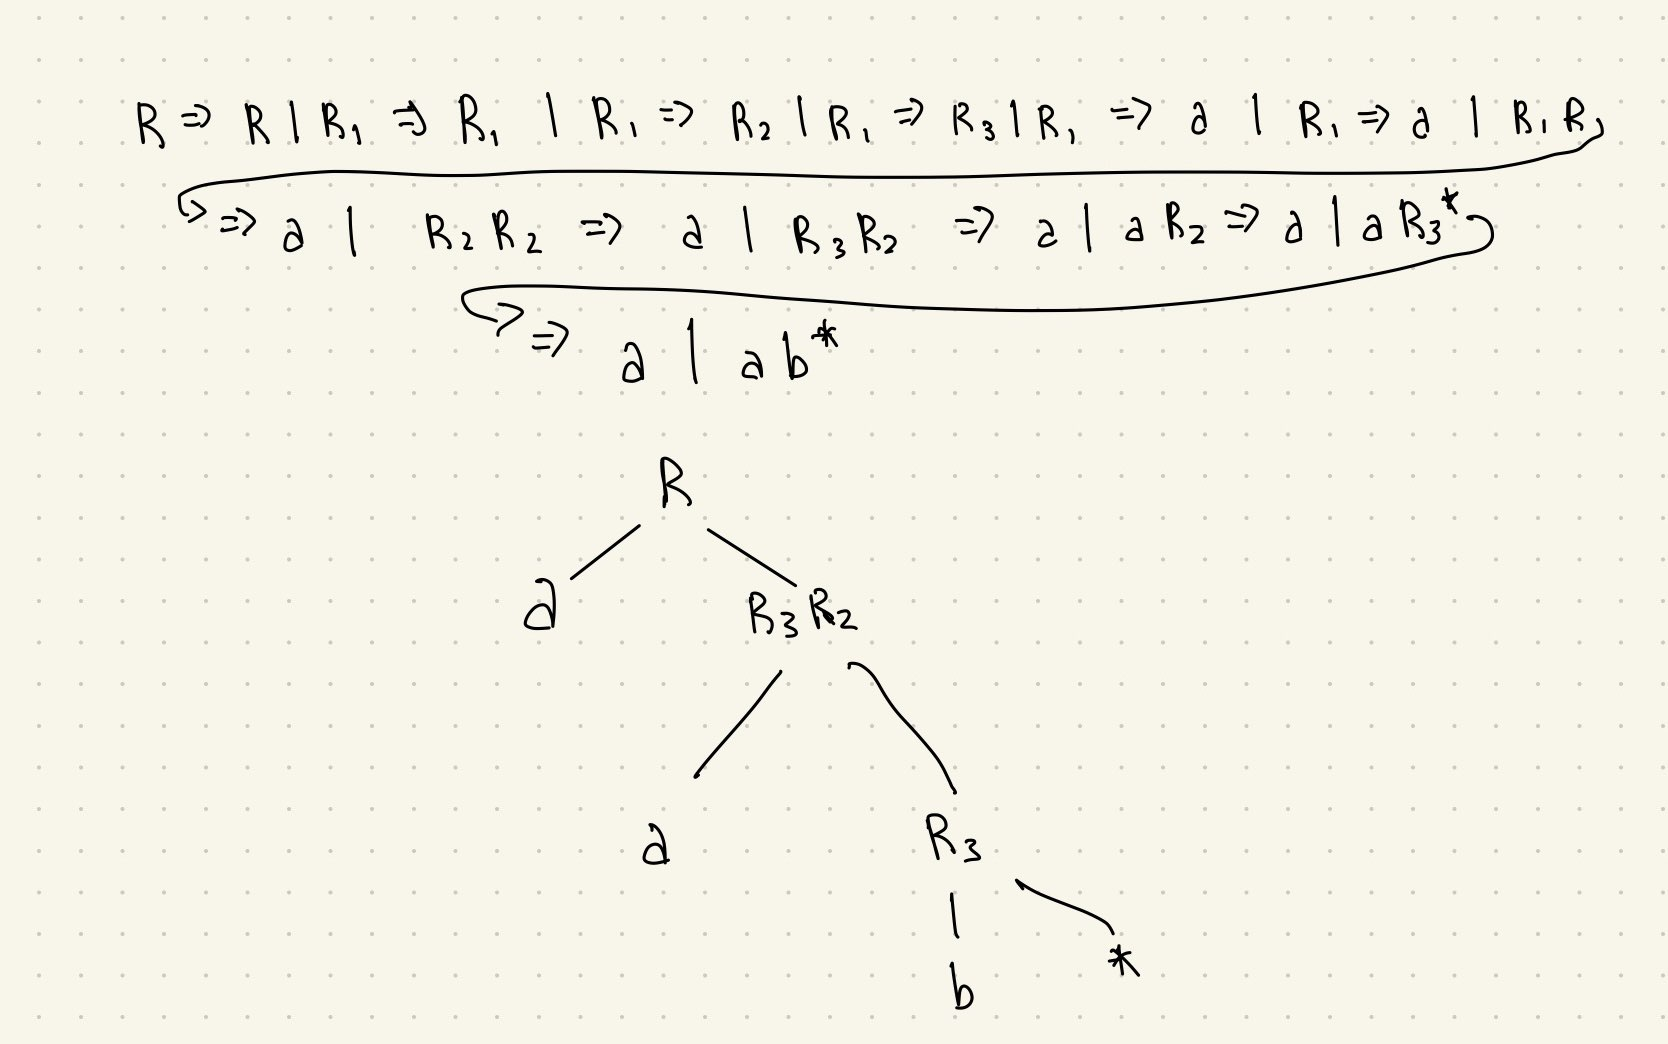
\includegraphics[width=0.6\textwidth]{IMG_0079.jpg}
\end{center}

\vspace{0.25cm}
\newpage
\item[(c)](3pts) Disambiguate into a \emph{right recursive} grammar.

\vspace{0.25cm}

$R \rightarrow R_1 \mid R \mid R_1$

$R_1 \rightarrow R_2 R_1 \mid R_2$

$R_2 \rightarrow R_3 \mid R_3^*$

$R_3 \rightarrow a \mid b \mid (R)$

\begin{center}
	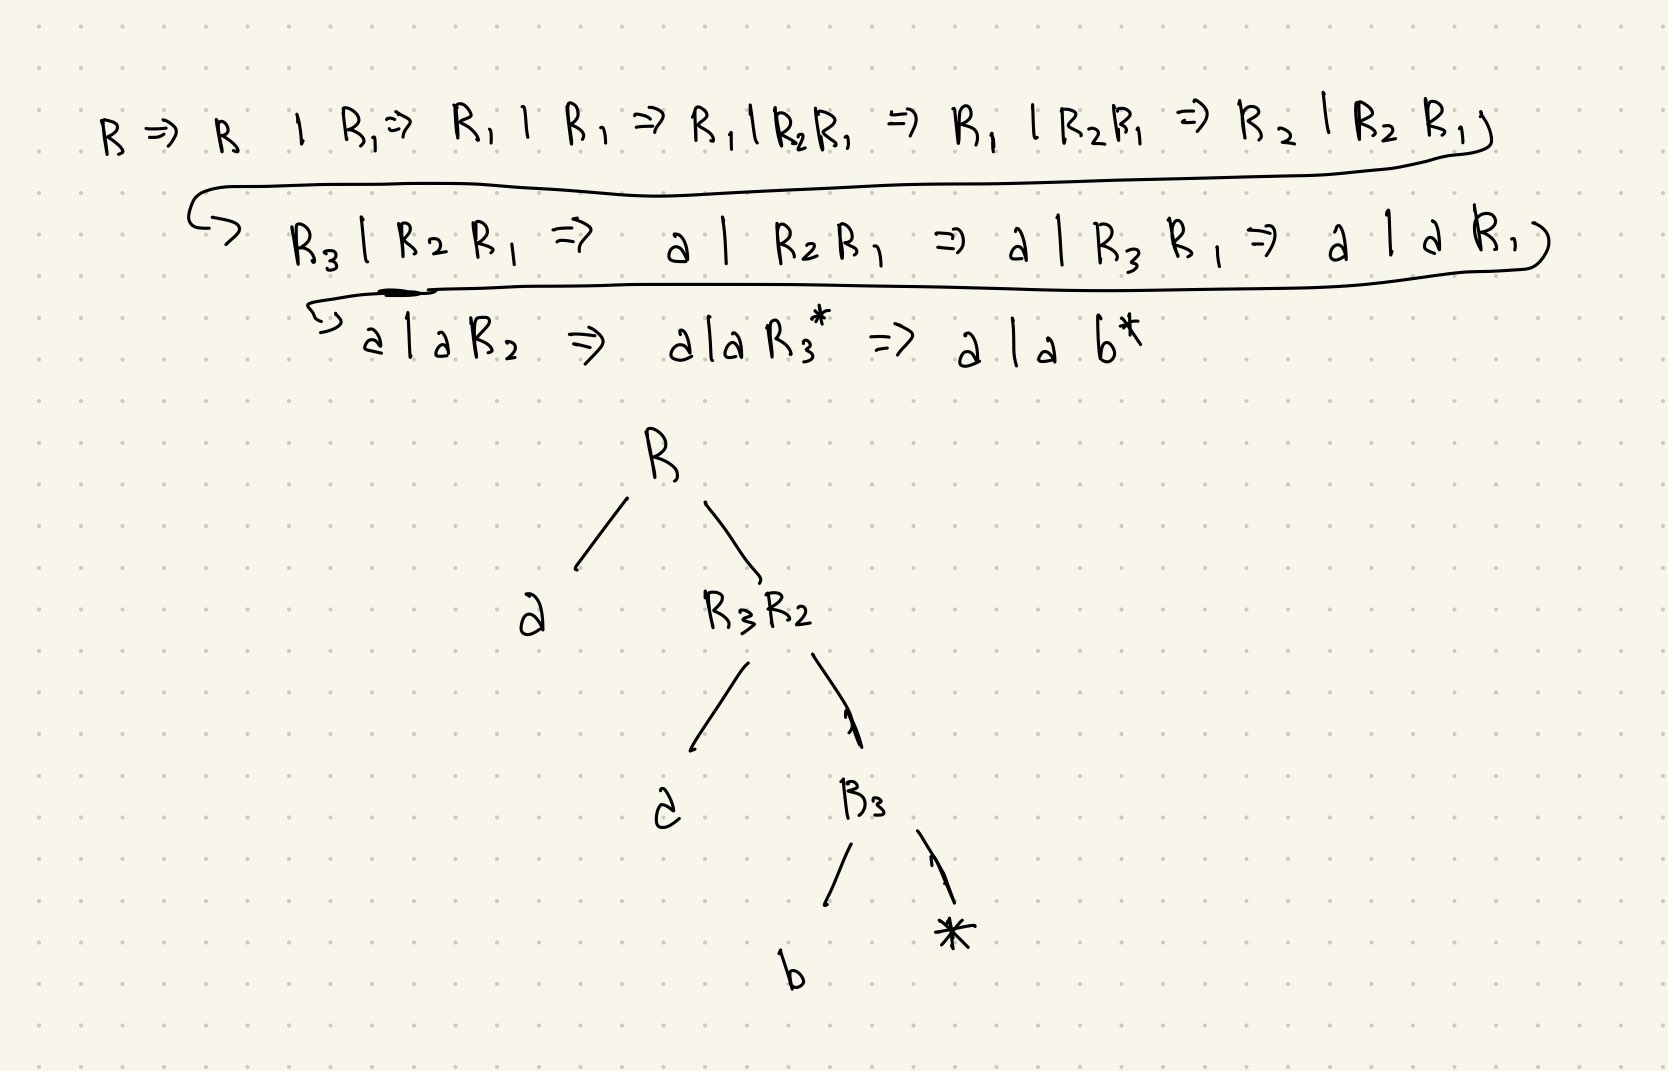
\includegraphics[width=0.6\textwidth]{IMG_0080.jpg}
\end{center}

\end{enumerate}

\vspace{0.15in}
\newpage

\noindent{\bf Problem 5.} Consider the following LL(1) grammar that generates S-expressions, an essential structure in Lisp-like languages. $S$ and $\mathit{Ss}$ are the nonterminals, \texttt{num} (number), \texttt{sym} (symbol), \texttt{(} and \texttt{)} are the terminals, i.e., the tokens.  
\[
\begin{array}{lll}
\mathit{Start} & \rightarrow & S\ \texttt{\$\$}\\
S & \rightarrow & \texttt{num} \\
S & \rightarrow & \texttt{sym} \\
S & \rightarrow & \texttt{(} \ Ss \ \texttt{)} \\
Ss & \rightarrow & S \  Ss \\
Ss & \rightarrow & \epsilon 
\end{array}
\]

\begin{enumerate}

\item[(a)] (2.5pts) What is FOLLOW($Ss$)? FOLLOW($S$)? PREDICT($Ss \rightarrow \epsilon$)?

\vspace{0.25cm}

FOLLOW(Ss) = $\{ ) \}$

FOLLOW(S) = $\{ num, sym, (, ), \$\$ \}$

PREDICT($Ss \rightarrow \epsilon$) = $\{ ) \}$

\vspace{0.25cm}

\item[(b)] (2.5pts) Draw a parse tree for the string \texttt{( 5 ( a ) ) \$\$}. 

\vspace{0.25cm}

$num = 5, sym = a$

\vspace{.25cm}

\begin{center}
    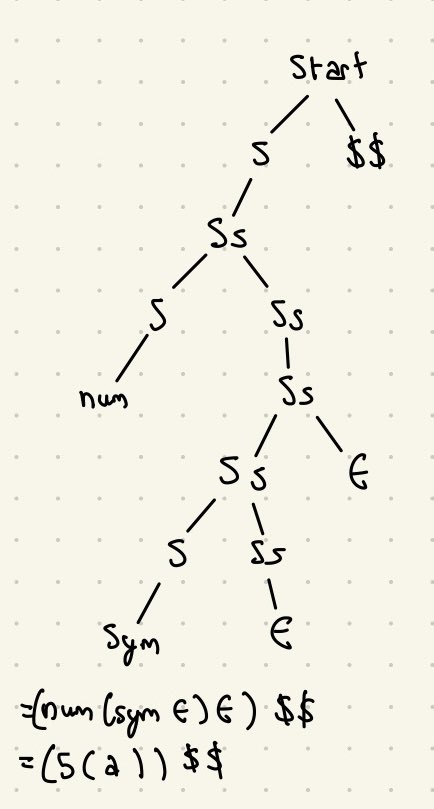
\includegraphics[width=0.3\textwidth]{IMG_0082.jpg}
\end{center}

\item[(c)] (3pts) Consider a recursive descent parser running on the same input. At the point
where token \texttt{a} is matched, which recursive descent routines will be 
active (i.e., what routines will have a frame on the run-time stack)?

\end{enumerate}

\vspace{.15in}

\newpage

\noindent{\bf Problem 6.} For each grammar below, determine if it is LL(1) or not and if it is ambiguous or not. You do not need to justify your answer, just write YES or NO. As an example of the format for answers we are looking for: (x) LL(1): YES, Ambiguous: YES.

\vspace{.05in}

\begin{enumerate}

\item[(a)] (1pts) $A \rightarrow \texttt{0}\ A\ \texttt{1} \mid \texttt{0}\ \texttt{1}$

\item[(b)] (1pts) $A \rightarrow \texttt{+}\ A\ A \mid \texttt{*}\ A\ A \mid \texttt{a}$

\item[(c)] (1pts) $A \rightarrow A\ \texttt{(}\ A\ \texttt{)}\ A \mid \epsilon$ 

\item[(d)] (1pts) $A \rightarrow B\ \texttt{a} \mid \texttt{b}\ B\ \texttt{c} \mid \texttt{d}\ \texttt{c} \mid \texttt{b}\ \texttt{d}\ \texttt{c} \quad \quad B \rightarrow \texttt{d}$ 

\item[(e)] (1pts) $S \rightarrow C\texttt{a}C\texttt{b} \mid D\texttt{b}D\texttt{a} \quad\quad C \rightarrow \epsilon \quad\quad D \rightarrow \epsilon$

\end{enumerate}

\vspace{0.25cm}

\begin{enumerate}
	\item [(a)] LL(1): NO, Ambiguous: NO
	\item [(b)] LL(1): YES, Ambiguous: NO	
	\item [(c)] LL(1): NO, Ambiguous: YES
	\item [(d)] LL(1): NO, Ambiguous: YES
	\item [(e)] LL(1): YES, Ambiguous: NO
	
\end{enumerate}


\end{document}